\documentclass{beamer}
\usepackage[spanish]{babel}
\usepackage{graphicx}
\usepackage{xcolor}
\usepackage{latexsym}
\usepackage{amsmath}
\usepackage{amssymb}
\usepackage{multicol}
\usepackage{tikz}

\usetheme{Boadilla}

\newtheorem{Teorema}{Teorema}

\definecolor{myblue}{RGB}{80, 69, 190} 

\setlength{\parskip}{0.1cm}

\newcommand{\indc}[4]{
    \begin{frame}
        \frametitle{Índice - Modelos NoSQL}
        	\begin{enumerate}
            \setbeamercovered{transparent}
            \item<#1> Clave-Valor  
            \item<#2> Columnar      
            \item<#3> Documental    
            \item<#4> Grafo
        \end{enumerate}
    \end{frame}
}

\newcommand{\estindc}[2]{
    \begin{frame}
        \frametitle{Índice - Articulos}
        	\begin{enumerate}
            \setbeamercovered{transparent}
            \item<#1> Assessment of SQL and NoSQL Systems to Store and Mine COVID-19 Data. 
            \item<#2> Performance investigation of selected SQL and NoSQL databases.
        \end{enumerate}
    \end{frame}
}

\newcommand{\myref}[2]{
    {\color{blue}\href{#1}{#2}}
}

\newcommand{\mytitle}[4]{
    \centering
    \vspace{0.1cm}
    
    {\Large \color{myblue} #1}

    \vspace{0.1cm}

    {\Large \color{myblue} #2}
    
    \vspace{0.5cm}
    
    {#3}
    
    \vspace{0.5cm}
    
    {\color{gray} #4}
    
    \vspace{0.5cm}
    
    {\today}
}

\title{Bases de datos NoSQL}
\author{Arroyo Joaquin \\ Belmonte Marina}

\begin{document}

\begin{frame}
    \mytitle
    {Bases de datos NoSQL}
    {Clase 2}
    {Arroyo Joaquin \\ Belmonte Marina}
    {Universidad Nacional de Rosario \\ Licenciatura en Ciencias de la Computación \\ Bases de Datos Avanzadas}
\end{frame}

\section{Resumen}
\begin{frame}
    \frametitle{Resúmen}

    \begin{itemize}
        \item Repaso de Modelos NoSQL

         
        
        \item Implementaciones de Modelos NoSQL

        \begin{itemize}
            \item Redis
            \item Apache HBase
            \item MongoDB
            \item Neo4j
        \end{itemize}

         
        
        \item Dos artículos que estudian el rendimiento de bases de datos SQL versus NoSQL en aplicaciones reales
    \end{itemize}
    
\end{frame}

\section{Repaso}
\begin{frame}
    \frametitle{Repaso}
    Como vimos en la clase 1, existe una amplia variedad de modelos de datos \textit{NoSQL}. Entre los más conocidos encontramos: 
    
     
    
    \begin{enumerate}
        \item Clave-Valor    
        \item Columnar        
        \item Documental     
        \item Grafo
    \end{enumerate}
\end{frame}

\section{Implementaciones}

\indc{1}{0}{0}{0}

\subsection{Clave-Valor}

\begin{frame}
    \frametitle{Clave-Valor - Repaso}

    Este modelo almacena pares del tipo (\textit{Key}, \textit{Value}).
    
    \begin{center}
    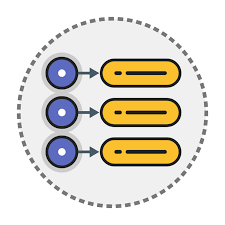
\includegraphics[width=0.2\textwidth]{images/KeyValue.png}
    \end{center}

     
    
     \begin{itemize}
        \item \textbf{Key}: Un identificador único para acceder al valor asociado.

         
        
         \item \textbf{Value}: Puede ser cualquier tipo de dato, desde texto, números y documentos, hasta listas o incluso otros pares clave-valor.
     \end{itemize}

\end{frame}

\begin{frame}
    \frametitle{Clave-Valor - Ejemplos}
    
    Algunas de las implementaciones más conocidas son:

     
    
     \begin{itemize}
        \item \textbf{Amazon DynamoDB}
                        
        \item \textbf{Voldemort}

        \item \textbf{Riak}
        
        \item \textbf{Redis}
     
     \end{itemize}

     

     Nos vamos a centrar en esta última.
\end{frame}

\subsubsection{Redis}

\begin{frame}   
    \frametitle{Clave-Valor - Redis}

    \textbf{Redis} significa ``\textbf{RE}mote \textbf{DI}ctionary \textbf{S}erver''

    \begin{center}
        
\includegraphics[width=0.3\textwidth]{images/redis_logo.png}
    \end{center}
    
     

    \begin{itemize}
        \item Base de datos de código abierto.  
        \item Rápida y versátil.  
        \item Diseñada como un almacén de estructuras de datos en memoria.
    \end{itemize}

\end{frame}

\begin{frame}
    \frametitle{Características de Redis}

    \begin{itemize}
        \item Estructuras de datos: strings, hashes, listas, conjuntos, etc.  
        \item Operaciones atómicas: Agregar, incrementar, intersección, unión, etc.  
        \item Replicación de datos incorporada.  
        \item Trabaja con un conjunto de datos en memoria.
    \end{itemize}
\end{frame}

\begin{frame}{Operaciones de Redis}
    
    Redis ofrece más de \textbf{400} operaciones e implementa la interfaz teórica para cada uno de los tipos de datos mencionados.
    
      

    Algunos ejemplos son:

      

    \begin{itemize}
        \item \textit{Strings:} $SET$, $GET$ y $DEL$
        
        \item \textit{Hashes:} $HSET$, $HGET$ y $HDEL$

        \item \textit{Listas:} $LPUSH$, $LPOP$, $RPUSH$, $RPOP$, $LRANGE$

        \item etc.
    \end{itemize}

\end{frame}

\begin{frame}{Ejemplo de Uso}
    \textbf{SET}: Agrega un par $(key, value)$.
    \begin{itemize}
        \item Complejidad temporal: $\mathcal{O}(1)$.
    \end{itemize}
    \vspace{0.6}
    \texttt{redis> SET subject1 "Base de Datos Avanzadas"} \newline
    \texttt{OK}   

\end{frame}
\begin{frame}{Ejemplo de Uso}
    \textbf{GET}: Obtiene el valor de una $key$.
    \begin{itemize}
        \item Complejidad temporal: $\mathcal{O}(1)$.
    \end{itemize}

    \texttt{redis> GET subject1}\newline
    \texttt{"Base de Datos Avanzadas"}

\end{frame}


\begin{frame}{Ejemplo de Uso}
    \textbf{LPUSH}: Inserta valores en la cabeza de una lista.
    \begin{itemize}
        \item Complejidad temporal: $\mathcal{O}(N)$.
    \end{itemize}
    
    \texttt{redis> LPUSH mylist "NoSQL"} \newline
    \texttt{redis> LPUSH mylist "Datos"} \texttt{"De"} \texttt{"Bases"}

\end{frame}
\begin{frame}{Ejemplo de Uso}
    \textbf{LRANGE}: Retorna los elementos en un rango especificado de una lista.
    \begin{itemize}
        \item Complejidad temporal: $\mathcal{O}(S + N)$.
    \end{itemize}
    \texttt{redis> LRANGE mylist 0 2} \newline
    \texttt{1) "Bases"} \newline
    \texttt{2) "De"} \newline
    \texttt{3) "Datos"} 
\end{frame}

\indc{0}{1}{0}{0}

\begin{frame}
    \frametitle{Columnar}

    Las bases de datos orientadas a columnas almacenan datos verticalmente por columnas en lugar de horizontalmente por filas, permitiendo un acceso más eficiente a datos específicos.
    
    \begin{center}
        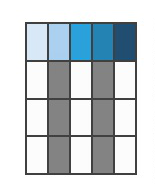
\includegraphics[width=0.3\textwidth]{diagramas/Columnar.png}
    \end{center}
\end{frame}


\begin{frame}
    \frametitle{Columnar - Ventajas}

    \begin{itemize}
        \item  Mayor eficiencia en consultas sobre columnas específicas.  
        \item  Convenientes para análisis de grandes volúmenes de datos.  
        \item  Adecuadas para aplicaciones de business intelligence y análisis predictivo.
    \end{itemize}
\end{frame}

\begin{frame}
    \frametitle{Columnar - Desventajas}
    \begin{itemize}
        \item  Operaciones de escritura más lentas debido a la reorganización de datos en columnas específicas.  
        \item  Posibles desafíos en entornos con datos altamente transaccionales.
    \end{itemize}
\end{frame}

\begin{frame}
    \frametitle{Columnar - Ejemplos}

    Algunos ejemplos de bases de datos columnares son: 
    
    \begin{itemize}
        \item \textbf{Apache Cassandra}\\
        Aunque es principalmente una base de datos de clave-valor, Cassandra utiliza un modelo de almacenamiento columnar para mejorar el rendimiento de ciertas consultas.  
        \item \textbf{Apache HBase}\\
        HBase es una base de datos de columnas distribuida, que almacena datos de forma columnar y permite un acceso eficiente a través de claves de fila.   
        \item \textbf{ClickHouse}\\
        ClickHouse es una base de datos de análisis columnar de código abierto diseñada para consultas analíticas de alto rendimiento en grandes conjuntos de datos.
    \end{itemize}
\end{frame}

\indc{0}{0}{1}{0}

\subsection{Documental}

\begin{frame}
    \frametitle{Documental}

    \begin{columns}
        \begin{column}{0.48\textwidth}
            Las bases de datos documentales almacenan datos en documentos individuales, que pueden ser estructurados o semi-estructurados como archivos JSON o XML.
        \end{column}
        \begin{column}{0.48\textwidth}
            \centering
            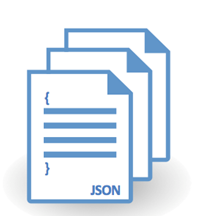
\includegraphics[width=0.5\textwidth]{images/Documental.png}
        \end{column}
    \end{columns}
    
     

    \vspace{0.3cm}
    
    Son especialmente adecuadas para aplicaciones donde los datos tienen una estructura flexible y variable como por ejemplo:

     
    
    \begin{itemize}
        \item \textbf{Contenido web}  
        \item \textbf{Análisis de registros}  
        \item \textbf{Gestión de datos de productos}
        \item etc.
    \end{itemize}
\end{frame}

\begin{frame}
    \frametitle{Documental - Ejemplos}

    Algunos ejemplos de bases de datos documentales son:
    
    \begin{itemize}
        \item \textbf{MongoDB}

        \item \textbf{CouchDB}
    \end{itemize}

     
    
    Nos vamos a centrar en MongoDB.
\end{frame}

\subsubsection{MongoDB}

\begin{frame}
    \frametitle{Documental - MongoDB}

        \centering
    
\includegraphics[width=0.4\textwidth]{images/mongodb-logo.png}
    \begin{itemize}
        \item Base de datos de código abierto, orientada a documentos y altamente escalable.  
        \item Desarrollada por MongoDB Inc.  
        \item Modelo de datos flexible basado en documentos BSON.  
        \item Utiliza almacenamiento basado en archivos de mapeo directo o motor WiredTiger.  
        \item Maneja replicación a través de conjuntos de réplicas para alta disponibilidad.  
        \item Distribuye datos en clústeres de servidores llamados fragmentos.  
        \item Lenguaje de consulta poderoso y flexible.
    \end{itemize}

\end{frame}

\begin{frame}[fragile]
\frametitle{Operaciones comunes en MongoDB}
\begin{itemize}
    \item \textbf{Insertar un documento}
    \begin{verbatim}
db.users.insertOne({
    name: "John Doe",
    age: 30,
    email: "john@example.com"
})

db.users.insertMany([
  { name: "Alice", age: 25 },
  { name: "Bob", age: 30 },
  { name: "Charlie", age: 50 }
])
    \end{verbatim}

\end{itemize}
\end{frame}

\begin{frame}[fragile]
\frametitle{Operaciones comunes en MongoDB}
\begin{itemize}
    \item \textbf{Consultar documentos}
    \begin{verbatim}
db.users.find({ age: { $gt: 25 } })
    \end{verbatim}

     
    \item \textbf{Actualizar documentos}
    \begin{verbatim}
db.users.updateOne(
    { name: "John Doe" },
    { $set: { age: 35 } }
)

db.users.updateMany(
    { status: "active" }, 
    { $set: { status: "inactive" } }
)

    \end{verbatim}
\end{itemize}
\end{frame}

\begin{frame}[fragile]
\frametitle{Operaciones comunes en MongoDB}
\begin{itemize} 
    \item \textbf{Eliminar documentos}
    \begin{verbatim}
db.users.deleteOne({ name: "John Doe" })
db.users.deleteMany({ age: { $gt: 40 } })
    \end{verbatim}
         
    \item \textbf{Contar documentos}
\begin{verbatim}
db.users.countDocuments({ age: { $lt: 30 } })
\end{verbatim}
         
    \item \textbf{Valores Distintos}
\begin{verbatim}
db.users.distinct("city", { country: "USA" })
\end{verbatim}
         
    \item \textbf{Agregar datos}
\begin{verbatim}
db.sales.aggregate([
  { $match: { status: "completed" } },
  { $group: { _id: "$product", 
            totalAmount: { $sum: "$amount" } } }
])
\end{verbatim}

\end{itemize}

\end{frame}

\indc{0}{0}{0}{1}

\subsection{Grafo}

\begin{frame}
    \frametitle{Grafo - Repaso}

    Las bases de datos en grafo utilizan estructuras de grafo para almacenar, consultar y relacionar datos. 

     
    
    \begin{columns}
        \begin{column}{0.48\textwidth}
            Los datos se representan mediante nodos (entidades) y arcos (relaciones entre entidades).
        \end{column}
        \begin{column}{0.48\textwidth}
            \centering
            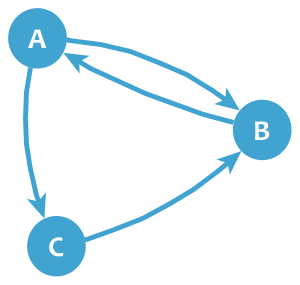
\includegraphics[width=0.4\textwidth]{images/Grafo.png}
        \end{column}
    \end{columns}

     

    \vspace{0.3cm}
    
    Pueden asignarse propiedades a nodos y arcos para capturar más detalles.

     
    
    Son ideales para almacenar datos interconectados.  

     
    
    Aplicaciones comunes incluyen: \textbf{Redes sociales}, \textbf{Sistemas de recomendación}, \textbf{Redes de trasportes}, etc.

    
\end{frame}

\begin{frame}
    \frametitle{Grafo - Ejemplos}

    Algunos ejemplos de bases de datos en grafos son:

    \begin{itemize}
        \item \textbf{Neo4j}\\
         
        \item \textbf{GraphBase}\\ 

        \item \textbf{Infinite Graph}\\
        
        \item \textbf{FlockDB}\\
    \end{itemize}
    
     

    Nos vamos a centrar en Neo4j.
    
\end{frame}

\subsubsection{Neo4j}

\begin{frame}
    \frametitle{Grafo - Neo4j}

    \centering
    
\includegraphics[width=0.5\textwidth]{images/neo4j-logo.png}

    \begin{itemize}
        \item Plataforma líder en bases de datos de grafos.  
        \item Diseño nativo de grafo para un rendimiento óptimo y escalabilidad excepcional.  
        \item Utiliza Cypher como su lenguaje de consulta principal.  
        \item Ofrece una interfaz integrada de visualización de grafos.  
        \item Altamente escalable y diseñado para manejar grandes volúmenes de datos.  
        \item Garantiza propiedades ACID.  
        \item Edición empresarial.
    \end{itemize}
    
\end{frame}

\begin{frame}{Cypher: Lenguaje de Consulta de Neo4j}
    \begin{itemize}
        \item Sintaxis intuitiva y expresiva.  
        \item Orientado a patrones.  
        \item Declarativo.  
        \item Soporte completo para operaciones CRUD.  
        \item Amplio soporte para funciones y operadores para operaciones avanzadas.
    \end{itemize}
\end{frame}

\begin{frame}
    \frametitle{Operaciones Básicas de Neo4j}

    Estas son algunas de las cláusulas básicas más comunes en Cypher y su sintaxis asociada:

     

    \begin{itemize}
        \item \textbf{Crear nodos y relaciones}

        \texttt{CREATE (a:Person \{name: 'John', age: 30\})} \newline
         
        \texttt{CREATE (b:Person:Employee 
                            \{name: 'Alice', role: 'Manager'\})}\newline
         
        \texttt{CREATE (a)-[:FRIENDS\_WITH]->(b)}

         
            
        \item \textbf{Especificar patrones}
        
        \texttt{MATCH (p:Person \{name: 'John'\}) RETURN p}\newline
         
        \texttt{MATCH (p:Person \{name: 'John'\})-[r]->() RETURN p, r}

         
    
    
        \item \textbf{Filtrar resultados}

        \texttt{WHERE n.name = 'John' AND friend.age > 25}

 
    \end{itemize}
    
\end{frame}

\begin{frame}
    \frametitle{Operaciones Básicas de Neo4j}


    \begin{itemize}

     
        \item \textbf{Devolver datos}

        \texttt{RETURN n, friend}

         
         
        \item \textbf{Actualizar propiedades}

        \texttt{SET n.age = 30}

         
        
        \item \textbf{Eliminar nodos y relaciones.}

        \texttt{DELETE n, friend}

         
            
        \item \textbf{Ordenar resultados}

        \texttt{ORDER BY n.name DESC}

         
        
        \item \textbf{Limitar número de resultados}

        \texttt{LIMIT 10}

         

        \item \textbf{Crear índices}

        \texttt{CREATE INDEX ON :Person(name)}
    
        
    \end{itemize}
    
\end{frame}

\begin{frame}[fragile]
  \frametitle{Ejemplo de Consulta en Neo4j}
      Para una demostración de como estas operaciones podrían ser utilizadas, supongamos que queremos encontrar los amigos en común entre dos usuarios en una red social y alguna información adicional sobre esos amigos en común:  
    \begin{verbatim}
MATCH (userA:User {username: 'UsuarioA'})
    -[:FRIENDS_WITH]-(commonFriend)-[:FRIENDS_WITH]-
    (userB:User {username: 'UsuarioB'})
RETURN commonFriend.username AS commonFriendUsername,
       commonFriend.age AS commonFriendAge
    \end{verbatim}

        
\end{frame}

\begin{frame}{Empresas que Utilizan Neo4j}
    \begin{itemize}
        \item Walmart
        \item Volvo
        \item eBay
        \item Cisco
    \end{itemize}
\end{frame}

\section{Estudios}

\estindc{1}{0}

\subsection{Assessment of SQL and NoSQL Systems to Store and
Mine COVID-19 Data}

\begin{frame}
    \frametitle{Assessment of SQL and NoSQL Systems to Store and Mine COVID-19 Data}

    Este estudio fue llevado a cabo en el año 2022 por tres investigadores pertenecientes a los siguientes institutos

    \vspace{-0.3cm}
    
    \begin{center}
        \textit{Instituto de Ingeniería de Coimbra}$^1$, \textit{Centro de Informática y Sistemas de la Universidad de Coimbra}$^2$ e \textit{Instituto Tecnológico de São Paulo}$^3$
    \end{center}

    \vspace{-0.4cm}
    
    \begin{center}
        João Antas$^1$, Rodrigo Rocha Silva$^{2,3}$ y Jorge Bernardino$^{1,2}$
    \end{center}

    \vspace{-0.1cm}
    
    y tuvo como objetivo:

     

    \begin{itemize}
        \item Estudiar diferentes sistemas de bases de datos, con el fin de ayudar a seleccionar el más adecuado para almacenar, gestionar y minar datos relacionados con el COVID-19.

         
        
        \item Llevar a cabo un proceso de Minería de Datos, empleando pruebas de clasificación de datos del software Orange Data Mining.
    \end{itemize}

     

    Nos vamos a centrar en mostrar como se logró el primer objetivo.
\end{frame}

\begin{frame}
    \frametitle{Assessment of SQL and NoSQL Systems to Store and Mine COVID-19 Data}

    Para ambos experimentos, utilizaron una computadora con las siguiente características:

     
    
    \begin{itemize}
        \item Windows 10
        \item Procesador Intel Core i7-8750H 2.20GHz
        \item 16 GB de RAM
        \item 256 GB SSD de Almacenamiento
    \end{itemize}

     
    
    Además las versiones de las tecnologías utilizadas fueron las siguientes:

     
    
    \begin{itemize}
        \item SQL Server versión 2017
        \item MongoDB versión 4.4
        \item Cassandra versión 3.11.10
    \end{itemize}
\end{frame}

\begin{frame}
    \frametitle{Assessment of SQL and NoSQL Systems to Store and Mine COVID-19 Data}

    Los datos fueron obtenidos de distintas fuentes, como hospitales, datos públicos, etc., y fueron almacenados en formatos CSV o XML antes de ser incorporados a las bases de datos.   Y para evaluar la escalabilidad de las bases de datos, crearon dos datasets de distintos tamaños. 

     
    
    Para el primer experimento, utilizaron seis queries diferentes, con el objetivo de evaluar el tiempo de ejecución, la RAM utilizada y el porcentaje de CPU de cada consulta. 
    
     
    
    Vamos a mostrar los resultados obtenidos sobre las consultas 1, 2 y 3, que se presentan a continuación.

\end{frame}

\begin{frame}
    \frametitle{Assessment of SQL and NoSQL Systems to Store and Mine COVID-19 Data}

    \begin{figure}[H]
        \begin{center}
            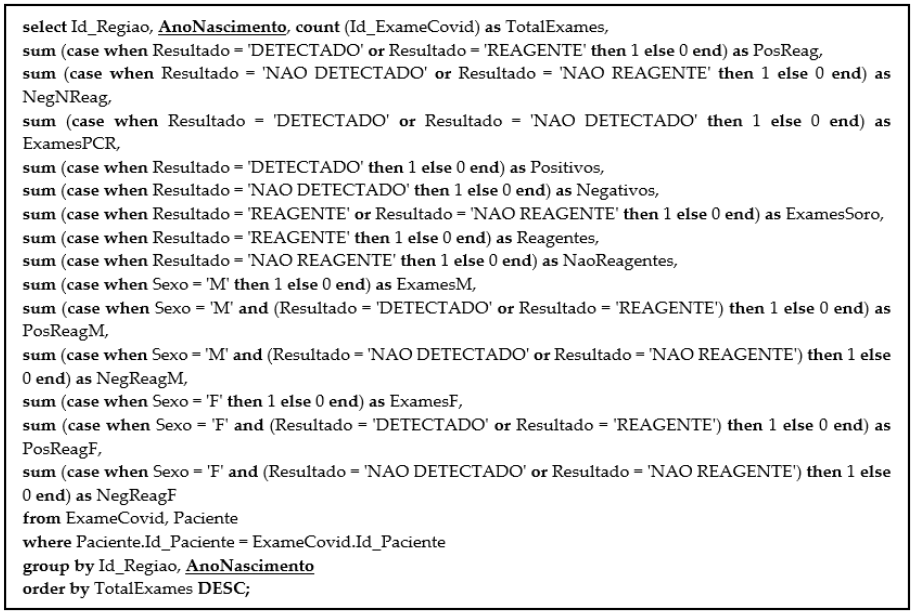
\includegraphics[width=0.7\textwidth]{images/cov19-query12.png}
            \caption{Query Region (Query 1 - sin subrayado) y Query RegionYear (Query 2)}
            \label{cov19-q12}
        \end{center}
    \end{figure}
\end{frame}

\begin{frame}
    \frametitle{Assessment of SQL and NoSQL Systems to Store and Mine COVID-19 Data}

    Esta query fue seleccionada utilizando un registro de auditoría que controlaba todas las consultas realizadas en la base de datos de SQL Server.
    
    \begin{figure}[H]
        \begin{center}
            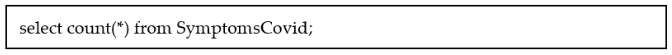
\includegraphics[width=0.82\textwidth]{images/cov19-query3.png}
            \caption{Query de Orange Data Mining (Query 3)}
            \label{cov19-q3}
        \end{center}
    \end{figure}
\end{frame}

\begin{frame}
    \frametitle{Assessment of SQL and NoSQL Systems to Store and Mine COVID-19 Data}

    \begin{figure}[H]
        \centering
        \begin{minipage}[b]{0.48\textwidth}
            \centering
            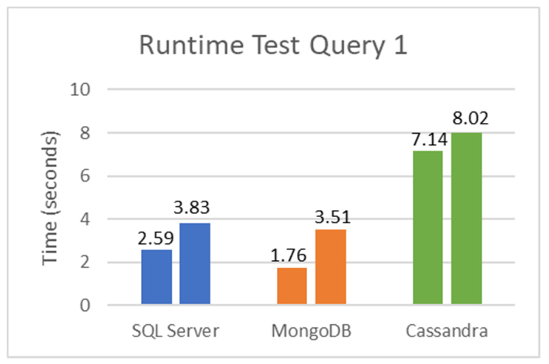
\includegraphics[width=\textwidth]{images/cov19-runt-test-q1.png}
            \caption{Prueba de tiempo de ejecución para la Query 1.}
        \end{minipage}
        \hfill
        \begin{minipage}[b]{0.48\textwidth}
            \centering
            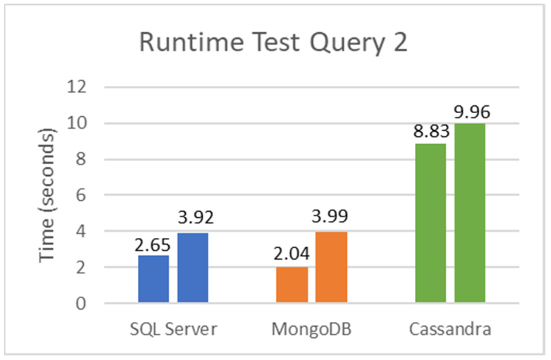
\includegraphics[width=\textwidth]{images/cov19-runt-test-q2.png}
            \caption{Prueba de tiempo de ejecución para la Query 2.}
        \end{minipage}
    \end{figure}
\end{frame}

\begin{frame}
    \frametitle{Assessment of SQL and NoSQL Systems to Store and Mine COVID-19 Data}

    \begin{figure}[H]
        \centering
        \begin{minipage}[b]{0.48\textwidth}
            \centering
            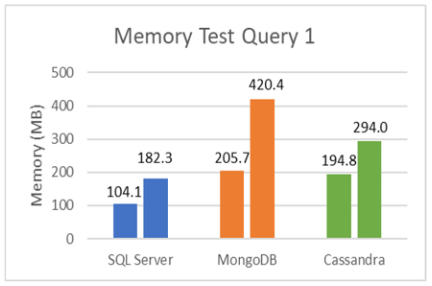
\includegraphics[width=\textwidth]{images/cov19-mem-test-q1.png}
            \caption{Memoria RAM utilizada para la Query 1.}
            \label{cov19-memtest-q1}
        \end{minipage}
        \hfill
        \begin{minipage}[b]{0.48\textwidth}
            \centering
            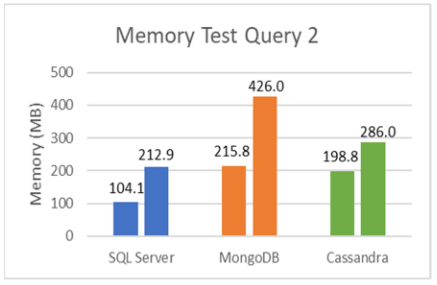
\includegraphics[width=\textwidth]{images/cov19-mem-test-q2.png}
            \caption{Memoria RAM utilizada para la Query 2.}
            \label{cov19-memtest-q2}
        \end{minipage}
    \end{figure}
\end{frame}

\begin{frame}
    \frametitle{Assessment of SQL and NoSQL Systems to Store and Mine COVID-19 Data}

    \begin{figure}[H]
        \centering
        \begin{minipage}[b]{0.48\textwidth}
            \centering
            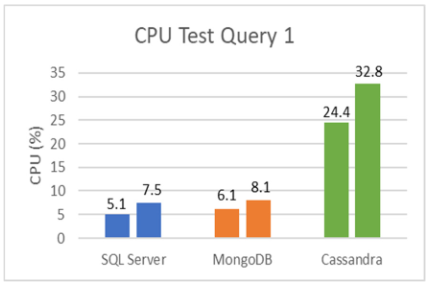
\includegraphics[width=\textwidth]{images/cov19-cpu-test-q1.png}
            \caption{Porcentaje de CPU utilizado para la Query 1.}
            \label{cov19-cputest-q1}
        \end{minipage}
        \hfill
        \begin{minipage}[b]{0.48\textwidth}
            \centering
            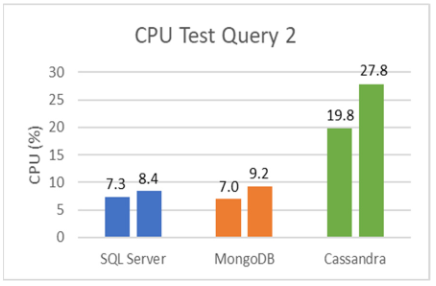
\includegraphics[width=\textwidth]{images/cov19-cpu-test-q2.png}
            \caption{Porcentaje de CPU utilizado para la Query 2.}
            \label{cov19-cputest-q2}
        \end{minipage}
    \end{figure}
\end{frame}

\begin{frame}
    \frametitle{Assessment of SQL and NoSQL Systems to Store and Mine COVID-19 Data}

    \begin{figure}[H]
        \centering
        \begin{minipage}[b]{0.48\textwidth}
            \centering
            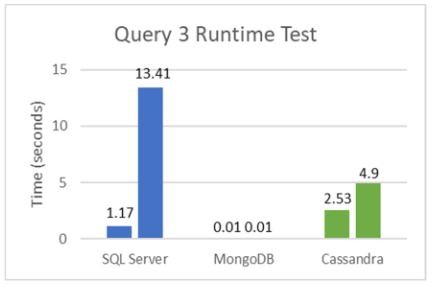
\includegraphics[width=\textwidth]{images/cov19-runt-test-q3.png}
            \caption{Prueba de tiempo de ejecución para la Query 3.}
            \label{cov19-runtest-q3}
        \end{minipage}
        \hfill
        \begin{minipage}[b]{0.48\textwidth}
            \centering
            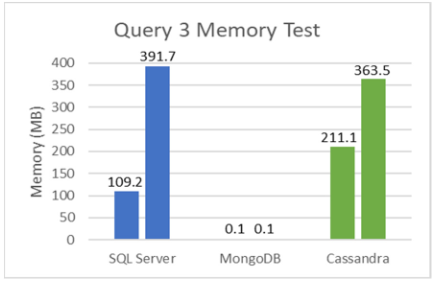
\includegraphics[width=\textwidth]{images/cov19-mem-test-q3.png}
            \caption{Memoria RAM utilizada para la Query 3.}
            \label{cov19-memtest-q3}
        \end{minipage}
    \end{figure}
\end{frame}

\begin{frame}
    \frametitle{Assessment of SQL and NoSQL Systems to Store and Mine COVID-19 Data}

    \begin{figure}[H]
        \centering
        \begin{minipage}[b]{0.48\textwidth}
            \centering
            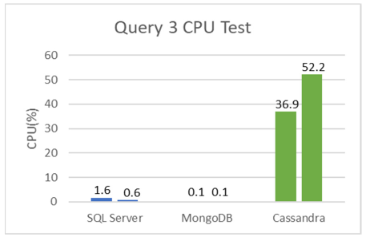
\includegraphics[width=\textwidth]{images/cov19-cpu-test-q3.png}
            \caption{Porcentaje de CPU utilizado para la Query 3.}
            \label{cov19-runtest-q3}
        \end{minipage}
        \hfill
        \begin{minipage}[b]{0.48\textwidth}
            \centering
            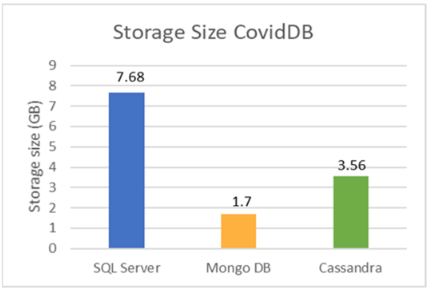
\includegraphics[width=\textwidth]{images/cov19-storage.png}
            \caption{Tamaño de la base de datos de COVID-19.}
            \label{cov19-memtest-q3}
        \end{minipage}
    \end{figure}
\end{frame}

\subsubsection{Conclusiones}

\begin{frame}
    \frametitle{Assessment of SQL and NoSQL Systems to Store and Mine COVID-19 Data - Conclusiones}

    Cabe destacar que los experimentos que no se mostraron, utilizaron consultas con \textit{joins}, y SQL Server tuvo un mejor rendimiento.

     

    \begin{itemize}
        \item SQL Server debería ser la elección si los datos son muy estructurados y necesitan consultas con \textit{joins}.

         
    
        \item Si se utiliza un gran volumen de datos no estructurados y no es necesario realizar demasiadas consultas con \textit{joins}, MongoDB o Cassandra se consideran las soluciones más adecuadas.
    \end{itemize}
\end{frame}

\estindc{0}{1}

\subsection{Performance investigation of selected SQL and NoSQL databases}

\begin{frame}
    \frametitle{Performance investigation of selected SQL and NoSQL databases}

    Este artículo fue presentado en el año 2015 en la Conferencia Internacional sobre Ciencia de la Información Geográfica (AGILE) por tres investigadores de la \textit{Universidad de Bundeswehr}:

     
    
    \begin{center}
        Stephan Schmid, Eszter Galicz y Wolfgang Reinhardt.
    \end{center}
    
     

    \begin{itemize}
        \item Trata sobre la creciente importancia de los datos espaciales, en el mundo actual.

         

        \item Explora las bases de datos NoSQL como una posible alternativa ante el dominio de las bases de datos relacionales para almacenar y manipular este tipo de datos.
    \end{itemize}
    
     
    
    Para los experimentos utilizaron tres bases de datos:

    \begin{center}
        \textbf{PostgreSQL}, \textbf{MongoDB} y \textbf{CouchBase}.
    \end{center}
\end{frame}

\begin{frame}
    \frametitle{Performance investigation of selected SQL and NoSQL databases}

    Para la representación de datos espaciales en PostgreSQL utilizaron \textbf{PostGis},   y en las dos siguientes utilizaron el formato \textbf{GeoJSON}, el cuál permite representar \textbf{Geometrías} (Puntos, Polígonos, Colección de Geometrías, etc.), \textbf{Características} y \textbf{Coleciones de Características}.

     

    Mencionan que al utilizar las estructuras de datos GeoJSON, el enfoque sin esquemas tiene algunas restricciones.
    
     
    
    Sin embargo, la representación geográfica debe seguir dicha estructura para poder establecer un índice geoespacial.
    
\end{frame}

\begin{frame}
    \frametitle{Performance investigation of selected SQL and NoSQL databases}

    Para los experimentos, los autores utilizaron una computadora con las siguientes características:

    \begin{itemize}
        \item Microsoft Windows Server 2008 R2
        \item 8 core CPU 2,5 GHz
        \item 10GB RAM
    \end{itemize}

     
    
    Utilizaron tres datasets para los experimentos, los cuales fueron obtenidos OpenStreetMap.

     
    
    \begin{table}[h]
        \centering
        \begin{tabular}{ |c|c|c| }
        \hline
        Level & Region & Size \\ 
        \hline
        Subregion & Niederbayern & 38.9 MB \\
        State & Bayern & 501 MB \\ 
        Country & Germany & 2.1 GB \\
        \hline
        \end{tabular}
        \caption{Datos de prueba utilizados de OpenStreetMap.}
    \end{table}
    
\end{frame}

\begin{frame}
    \frametitle{Performance investigation of selected SQL and NoSQL databases}
    
    \begin{minipage}{0.55\textwidth}

        Y eligieron dos tipos de consultas para el análisis:

        \begin{enumerate}
            \item Consultas sobre información de atributos.
    
            \item Consultas que utilizan la geo-función \textit{within}.
        \end{enumerate}
        
        \begin{figure}
            \centering
            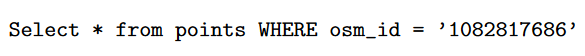
\includegraphics[width=\textwidth]{images/geo_q1.png}
            \caption{Query 1}
        \end{figure}
    \end{minipage}\hfill
    \begin{minipage}{0.43\textwidth}
        \begin{figure}
            \centering
            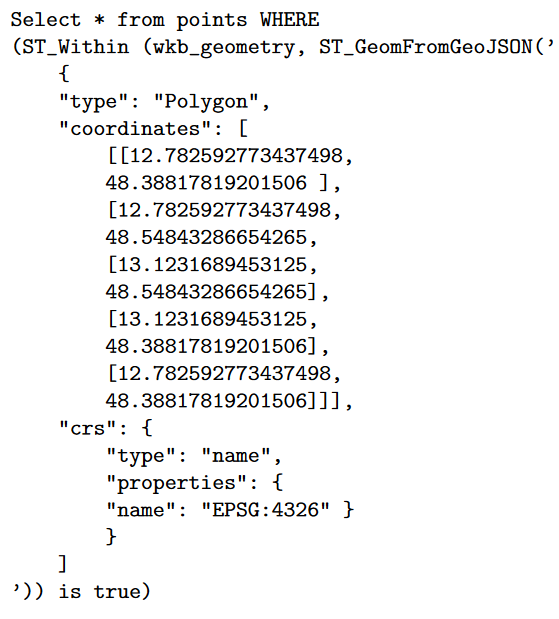
\includegraphics[width=\textwidth]{images/geo_q2.png}
            \caption{Query 2}
        \end{figure}
    \end{minipage}
    
\end{frame}

\begin{frame}
    \frametitle{Performance investigation of selected SQL and NoSQL databases}

    Para realizar la simulación en condiciones realistas, las consultas se realizaron con una determinada cantidad de usuarios, la cuál va en aumento:

    \vspace{-0.4cm}
    
    \begin{center}
        100, 250 y 500 usuarios.
    \end{center}

     

    \begin{minipage}{0.48\textwidth}
        \begin{figure}
            \centering
            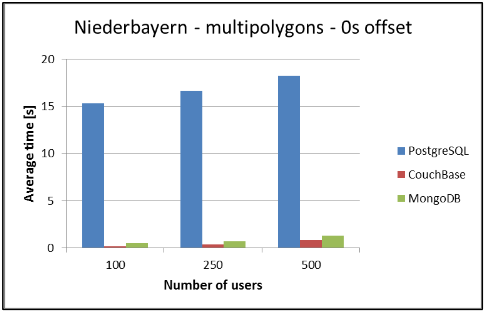
\includegraphics[width=\textwidth]{images/geo-g1.png}
            \caption{Resultados Query 1}
        \end{figure}
    \end{minipage}\hfill
    \begin{minipage}{0.48\textwidth}
        \begin{figure}
            \centering
            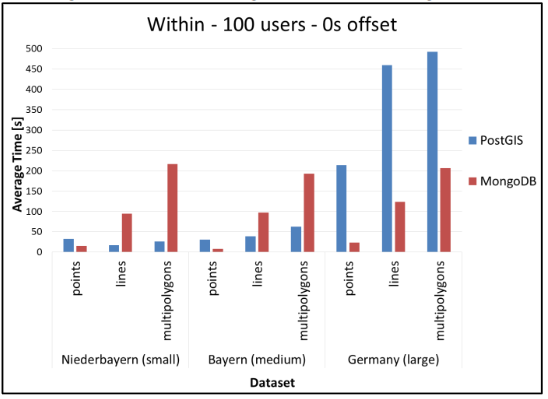
\includegraphics[width=\textwidth]{images/geo-g2.png}
            \caption{Resultados Query 2}
        \end{figure}
    \end{minipage}
\end{frame}

\subsubsection{Conclusiones}

\begin{frame}
    \frametitle{Performance investigation of selected SQL and NoSQL databases - Conclusión}

    \begin{itemize}
        \item Las consultas con el uso de geo-funciones llevan más tiempo que las consultas sobre información de atributos.

         
        
        \item Para solicitudes puramente sobre información de atributos, las bases de datos NoSQL son superiores en comparación con las bases de datos SQL.

         
        
        \item Los resultados muestran claramente que las bases de datos NoSQL son una alternativa posible, al menos para consultar información de atributos.
    \end{itemize}
\end{frame}

\section{Dudas}

\begin{frame}
    \vspace{1cm}
    
    \centering
    Dudas?
\end{frame}

\section{Referencias}
\begin{frame}
\frametitle{Referencias}
    \begin{itemize}
    	\item[1] \myref{https://redis.io/es/}{redis.io} Accedido el 15.04.2024

        \item[2] \myref{https://hbase.apache.org/}{hbase.apache.org} Accedido el 13.05.2024

        \item[3] \myref{https://www.mongodb.com/es}{mongodb.com} Accedido el 13.05.2024
        
        \item[4] \myref{https://neo4j.com/}{neo4j.com} Accedido el 06.05.2024
        
        \item[5] Antas, J., Silva, R.R., Bernardino, J.: Assessment of sql and nosql systems to store and mine covid-19 data. MDP Comput. Suv. (2022)

        \item[6] Schmid, S., Galicz, E., Reinhardt, W.: Performance investigation of selected sql and nosql databases (2015)

        \item[7] \myref{https://datatracker.ietf.org/doc/html/rfc7946}{datatracker.ietf.org/doc} Accedido el 10.05.2024
        
    \end{itemize}
\end{frame}

\end{document}